\documentclass[tc]{texufpel}

\usepackage[brazilian]{babel}
\usepackage[utf8]{inputenc}
\usepackage[T1]{fontenc}
\usepackage{graphicx}
\usepackage{subfigure}
\usepackage{array}
%\usepackage{abntcite}
\usepackage{times}              % pacote para usar fonte Adobe Times
\usepackage{mathptmx}          % p/ usar fonte Adobe Times nas fórmulas
\usepackage{setspace}
	\onehalfspacing

\author{Giusti}{Filipe Vernetti}
\title{FERRAMENTA PARA AUXÍLIO AO DIAGNÓSTICO DE IMAGENS PULMONARES DE TOMOGRAFIA COMPUTADORIZADA}
\advisor[Prof.~Dr.]{Oliveira}{Lucas Ferrari}

\date{Dezembro}{2008}

\renewcommand{\nominata}{
        UNIVERSIDADE FEDERAL DE PELOTAS\\
        Reitor: Prof.~Dr.~Cesar Borges\\
        Coordenador do curso: Prof.~Dr.~Lucas Ferrari Oliveira\\
}

% TODO: keywords
\keyword{processamento de imagens}
\keyword{tomografia computadorizada}
\keyword{pulmão}

% Desencorajar fortemente a hifenização, já que não é permitido
\hyphenpenalty=6000
\tolerance=1000

\begin{document}

\maketitle

% TODO: examinadores
\examiner{Prof.~Dr.~Armando Multas}
\examiner{Prof\textsuperscript{a}.~Dr\textsuperscript{a}.~Nomelinda Longuinha da Silva Paes Netto}
\examiner{Prof.~MSc.~Gerúndio das Dores}
\makeexaminers

% Epígrafe
% TODO: frase de efeito
\clearpage
\begin{flushright}
\mbox{}\vfill
{\sffamily\itshape
``If I have seen farther than others,\\
it is because I stood on the shoulders of giants.''\\}
--- \textsc{Sir~Isaac Newton}
\end{flushright}

% Agradecimentos
% TODO: agradecimentos
\chapter*{Agradecimentos}
Agradeço ao \LaTeX\ por não ter vírus de macro\ldots

% Dedicatória
% TODO: dedicatoria
\chapter*{Dedicatoria}
Dedico esse trabalho a mim.
\begin{abstract}
Este trabalho apresenta o resultado do desenvolvimento de uma ferramenta que utiliza técnicas de processamento de imagens e redes neurais artificiais, com objetivo de facilitar o diagnóstico de exames de tomografia computadorizada pulmonar. Possui uma interface web a qual pode ser instalada em um servidor e utilizada de qualquer lugar. É um sistema que com a interação do usuário tem a capacidade de ir se adaptando e melhorando, pois é um sistema de recuperação de imagens baseada em conteúdo que leva em consideração o usuário. Este trabalho faz uso de redes neurais artificiais com topologia de pró-alimentação e algoritmo de retro-propagação para treinamento. Dessa forma o sistema pode aprender a similaridade entre duas imagens. A ferramenta desenvolvida nesse trabalho pode dimnuir a taxa de erros nos diagnósticos de um médico inexperiente.

\end{abstract}


\begin{englishabstract}{Application for computer aided diagnosis of computed tomography lung images}{image processing, computed tomography, artificial neural network, content based image retrieval}

This paper presents the result of the development of a tool that uses some techniques of image processing and artificial neural networks, aiming to facilitate the diagnosis of lung computed tomography examinations. It has a web interface which can be installed and used on a server from anywhere. It is a system that using the user's relevance feedback is capable of adjusting and improving itself, because it is a system of content based image retrieval. This work makes use of artificial neural networks with feedforward topology and back-propagation algorithm for training. Thus the system can learn the similarity between two images. The tool developed in this work can lower the erro rate in the diagnosis of an inexperienced doctor.
\end{englishabstract}

\listoffigures
\listoftables

\begin{listofabbrv}{SPMD}
	\item[2D] Bidimensional
	\item[3D] Tridimensional
	\item[TC] Tomografia Computadorizada
	\item[UH] Unidade Hounsfield
\end{listofabbrv}

%\begin{listofsymbols}{$\alpha\beta\pi\omega$}
%       \item[$\sum{\frac{a}{b}}$] Somatório do produtório
%       \item[$\alpha\beta\pi\omega$] Fator de inconstância do resultado
%\end{listofsymbols}

\tableofcontents

\chapter{Introdução}

O exame de tomografia computadorizada - TC - resulta em diversas imagens que representam secções do corpo. Elas são geradas através de uma sucessão de raios-x que são posteriormente processados por computador. Essas imagens podem ser reunidas de forma a se obter uma representação tridimensional - 3D - do corpo.

Ao analisar um exame de TC para realizar um laudo, o médico faz um julgamento subjetivo com base na sua experiência. Se o médico possuir pouca experiência e não estiver seguro o suficiente para emitir o laudo, terá de realizar uma busca pelas patologias que são mais prováveis e comparar a descrição encontrada com a imagem do paciente, apesar de que às vezes são encontradas descrições com algumas imagens de exemplo, comparar uma descrição textual com uma imagem é um processo muito suscetível à falhas.

O exame de TC gera muitas imagens a serem analisadas, e essa grande quantidade de imagens contribui enormemente para o aumento de falhas humanas, pois analisar diversas imagens é um processo trabalhoso, complexo e tedioso. O grande número possível de combinações de padrões complexos achados nas diversas imagens, a falta de correlação fortemente estabelecida entre os achados radiológicos e patológicos e variações na forma de interpretação e descrição dos achados radiológicos, sem uma definição objetiva, são os principais fatores que resultam em grandes variações entre diagnósticos \cite{uchiyama}.

Para tentar acelerar a análise e diminuir o número de laudos incorretos, foi desenvolvida uma ferramenta para auxiliar os médicos na tomada de decisão do laudo. Os resultados alcançados estão expostos nesse trabalho.

A ferramenta é capaz de processar e analisar a imagem do paciente, e então recuperar de uma base de conhecimento, imagens similares, dessa forma possibilitando ao médico a comparação visual com diversas outras imagens de TC. Das imagens similares é possível acessar o laudo emitido, criando assim mais subsídios para o médico na hora de emitir o diagnóstico.

\section{Motivação}

Tornar a avaliação de imagens de TC menos subjetiva, facilitando o trabalho de médicos menos experientes. Além de fornecer uma forma rápida de comparar exames similares de diferentes pacientes, tornando mais preciso o diagnóstico. Um dos propósitos de se desenvolver uma ferramenta como essa reside no fato de que, reconhecidamente, a avaliação desse tipo de doença é um dos problemas mais difíceis no diagnóstico médico \cite{doi}, \cite{bick}.

É importante evidenciar que a ferramenta desenvolvida é distribuída na forma de software livre, podendo, por isso, ser redistribuída, usada e modificada.

\section{Objetivos}

O objetivo desse trabalho é a realização de um estudo sobre técnicas de segmentação e extração de características de imagens pulmonares de TC e métodos para recuperação de imagens baseado em conteúdo, objetivando o desenvolvimento de um software capaz de auxiliar médicos no diagnóstico desse tipo de imagem.

O software desenvolvido realiza 3 etapas principais:
\begin{enumerate}
 \item Segmentação das imagens resultantes da TC, visando extrair as regiões de interesse, que são os pulmões, e separa-los. Um dos meios que surgiram para auxiliar na segmentação e registro de imagens médicas foi o framework ITK – Insight Segmentation and Registration Toolkit. Com o qual espera-se conseguir um desenvolvimento mais rápido do software \cite{yoo}.
 \item Criação do vetor de características para cada pulmão segmentado na etapa anterior.
 \item Comparação da imagem com outras previamente inseridas no software, utilizando uma função de similaridade.
\end{enumerate}

\section{Organização}

Este trabalho, dividido em sete capítulos, apresenta primeiramente os conceitos estudados durante o seu desenvolvimento, seguido da descrição da ferramenta desenvolvida, os resultados obtidos e as conclusões.

No segundo capítulo, é apresentada uma introdução sobre as imagens de TC pulmonar, assim como suas características relevantes, e um estudo sobre o método de segmentação utilizada.

No capítulo seguinte, são explicadas técnicas de extração de características.

No quarto capítulo, é demonstrado o funcionamento básico de um sistema de recuperação de imagens baseado em conteúdo.

No quinto capítulo, é descrito o software desenvolvido durante este trabalho, bem como as bibliotecas utilizadas.

No sexto capítulo são exibidos os resultados obtidos pela ferramenta desenvolvida e, no último capítulo, são apresentadas as conclusões e as sugestões de trabalhos futuros.
\chapter{Processamento de Imagens}

O processamento digital de imagens é um campo cujas aplicações são bastante extensas. Existem métodos de processamento de imagens para interesses muito diferentes, que vão desde a melhoria das informações visuais para a interpretação dos médicos até a computação dos dados da imagem para transmissão, armazenamento ou interpretação autônoma por computador \cite{gonzalez}.

O processamento digital de imagens médicas é uma área em grande evolução e uma das que mais representa desafios dentro do processamento de imagens. Mas apesar de ser objeto de pesquisas de várias instituições ao redor do mundo, são poucos os sistemas deste tipo utilizados na prática médica. O principal fator é que este tipo de sistema exige alta eficiência, pois deve ser rápido, para que o tempo de resposta ao paciente não seja grande e ter uma baixíssima taxa de erros. Seus resultados são utilizados para tomar decisões em termos de diagnóstico e escolha de tratamento, por isso, alguns tipos de erro são inadmissíveis.

Em geral, os sistemas de processamento de imagens médicas extraem informações que podem ser provenientes de diversos tipos de modalidades de imagens, como Radiografia, Ultra-sonografia e Ressonância Magnética Nuclear, entre outras. Além das técnicas de processamento de imagens, técnicas de inteligência artificial, reconhecimento de padrões, entre outras áreas computacionais, são também aplicadas com o objetivo de melhorar tais imagens e extrair delas informações úteis ao diagnóstico.

\section{Imagens de tomografia computadorizada}

A tomografia era um dos mais importantes métodos de diagnóstico radiológico até a invenção da tomografia computadorizada - TC, na década de 70 do século passado. Sendo um dos primeiros tipos de exame a se beneficiar da popularização da computação.

A utilização de imagens no campo da medicina tem como principal objetivo proporcionar uma avaliação não invasiva dos tecidos e órgãos do corpo humano, tornando possível a verificação de anormalidades causadas por doenças ou acidentes \cite{oliveira}.

As máquinas de TC possuem uma fonte de raios x e detectores de raios x, os quais ficam em lados opostos um do outro. Para construir as imagens de TC a fonte e os detectores de raios x são movidos para posições pre-determinadas e então obtem diversas imagens, como demonstrado \ref{fig:tc1}, as quais representam fatias finas do paciente.

\begin{figure}[ht]
 \begin{center}
  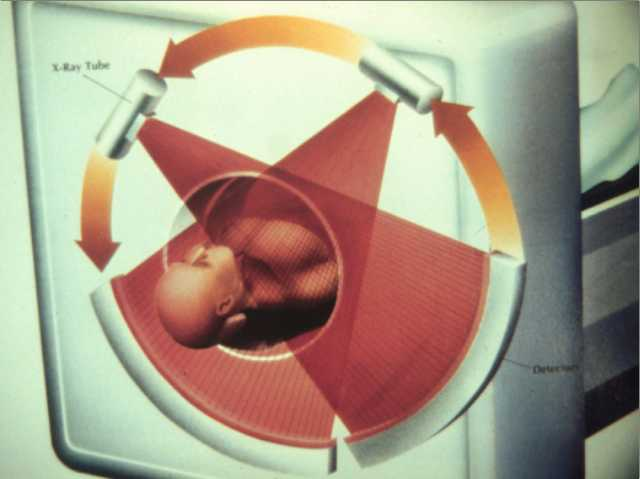
\includegraphics{imagens/tc.jpg}
 \end{center}
 \caption{Demonstração de como uma máquina de TC obtém as fatias de imagem do paciente.}
% TODO: referencia = http://www.sprawls.org/resources/CTIMG/classroom.htm
 \label{fig:tc1}
\end{figure}

A forma de movimentação depende da tecnologia da máquina utilizada. Nas máquinas mais antigas, eram tiradas várias fotos de uma fatia do paciente, apenas circulando em torno dele, e então depois a "cama" onde o paciente deita-se se move, para outra rodada de fotos, como em \ref{fig:tc2}. Hoje em dia, temos as máquinas helicoidais, os quais descrevem uma hélice em torno do paciente, em vez de uma sucessão de círculos completo. Desta forma é obtida informação de uma forma contínua.

\begin{figure}[ht]
 \begin{center}
  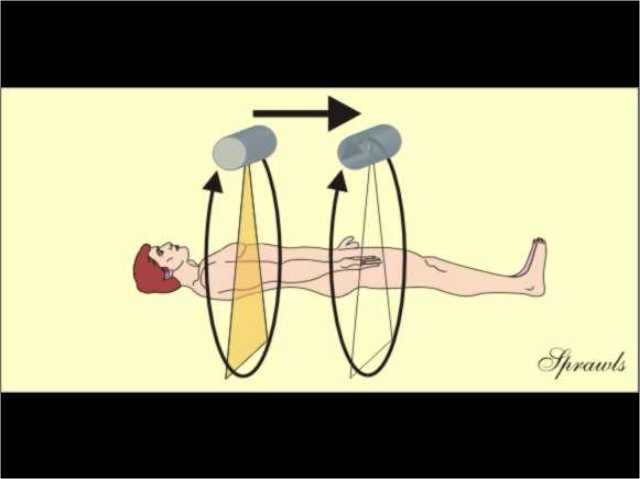
\includegraphics{imagens/tc2.jpg}
 \end{center}
 \caption{Forma de movimentação de máquinas de TC de tecnologia antiga.}
% TODO: referencia = http://www.sprawls.org/resources/CTIMG/classroom.htm
 \label{fig:tc2}
\end{figure}

O resultado de cada pixel das fatias obtidas é a soma das energias bloqueadas pelos tecidos do corpo, e sabe-se exatamente em que ângulo cada fatia foi tirada, por isso após a aquisição das seções transversais, é possivel a reconstrução da imagem em até 3 dimensões. Para a reconstrução é utilizada uma técnica matemática chamada de projeção retrógrada, ou outras, como a transformada de Fourier.

% TODO: expandir ou nao expandir? eis a questão.

Essas imagens são geralmente de 512x512 pixels, embora alguns equipamentos possuam uma resolução de 1024x1024 pixels. O tamanho do pixel é da ordem de 1mm, podendo chegar em algumas unidades a valores em torno de 0,1mm.
% TODO: referencia

\subsection{Coeficiente de Hounsfield}

A escala da unidade hounsfield - UH - é uma transformação linear da medida do coeficiente de atenuação linear original, do qual a radiodensidade da água destilada a temperatura e pressão ambientes é definida como 0 UH, enquanto a radiodensidade do ar a temperatura e pressão ambientes é -1000 UH. Para um material X com coeficiente de atenuação $\mu$X, o correspondente valor em unidades Hounsfiled é dado por \ref{equa:hounsfield}.

\begin{equation}
	\frac{\mu_X-\mu_{H_2O}}{\mu_{H_2O}-\mu_{ar}}\times 1000
	\label{equa:hounsfield}
\end{equation}

onde $\mu_{H_2O}$ e $\mu_{ar}$ são os coeficientes de atenuação linear da água e do ar, respectivamente, a pressão e temperatura ambientes. Então uma mudança de uma UH representa uma mudança de 0,1\% da diferença do coeficiente de atenuação entre a água e o ar, ou aproximadamente 0,1\% do coeficiente de atenuação da água, já que o coeficiente de atenuação do ar é aproximadamente 0. Alguns valores Hounsfield conhecidos estão mostrados na \ref{tab:hounsfield}.

\begin{table}
 \label{tab:hounsfield}
 \caption{Valores Hounsfield comuns.}
 \cite{oliveira} % TODO: funciona?
 \begin{center}
 \begin{tabular}{|l|r|}
 \hline
%TODO: trocar palavra tecido
 	\textbf{Tecido} & \textbf{Unidade Hounsfield} \\ \hline
 	Ar & -1000 \\ \hline
 	Pulmão & -900 a -400 \\ \hline
 	Gordura & -110 a -65 \\ \hline
 	Água & 0 \\ \hline
 	Rim & 35 \\ \hline
 	Sangue normal & 35 a 55 \\ \hline
 	Sangue coagulado & 80 \\ \hline
 	Músculo & 40 a 60 \\ \hline
 	Fígado & 50 a 85 \\ \hline
 	Ossos & 130 a 250 \\
 \hline
 \end{tabular}
 \end{center}
\end{table}

\subsection{Técnica de Janelas}

O olho humano tem a capacidade de diferenciar uma escala de cinzas de 10 a 60 tons (a maioria das pessoas distingue 20 diferentes tons), enquanto na tomografia há no mínimo 2000 tons. A técnica de janelas é na verdade uma forma de mostrar apenas uma faixa de tons de cinza que nos interessa, de forma a adaptar a nossa capacidade de visão aos dados obtidos pelo tomógrafo.
%TODO: referencia

Precisamos definir os valores máximo e mínimo da janela, para mapear os valores em UH em níveis de cinza. Todos os valores abaixo do valor mínimo serão mapeados como preto e todos acima do máximo como branco. Para definir estes valores, especificamos o tamanho da janela em UH e o centro dela, como podemos ver em \ref{fig:tc_janela}.

\begin{figure}[ht]
 \begin{center}
  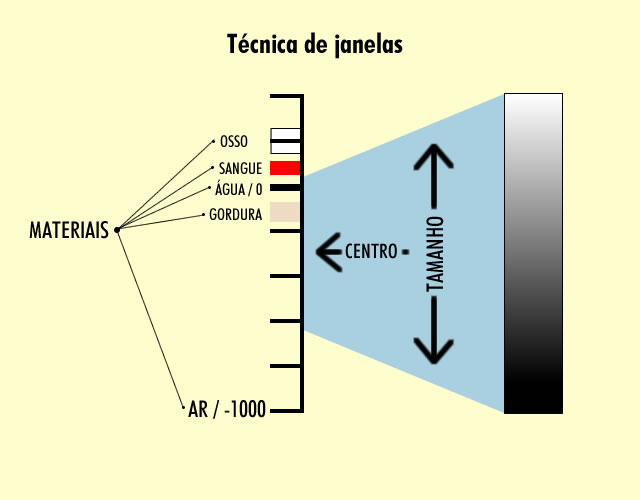
\includegraphics[height=3.0in]{imagens/tc_janela.jpg}
 \end{center}
 \caption{Exemplo de janela.}
%TODO: finalizar
 \label{fig:tc_janela}
\end{figure}

O uso de diferentes janelas em tomografia permite por exemplo o estudo dos ossos com distinção entre a cortical e a medular óssea ou o estudo de partes moles com a distinção, por exemplo, no cérebro entre a substância branca e a cinzenta. A mesma imagem pode ser mostrada com diferentes ajustes da janela, de modo a mostrar diferentes estruturas de cada vez. Não é possível usar um só ajuste da janela para ver, por exemplo, detalhes ósseos e de tecido adiposo ao mesmo tempo. Alguns valores comuns de janela estão na \ref{tab:janela}.

\begin{table}
 \label{tab:janela}
 \caption{Valores comuns de janela para certos tipos de exame.}
% TODO: referencia
% TODO: fazer tabela
 \begin{center}
 \begin{tabular}{|l|r|r|}
 \hline
 	\textbf{Exame} & \textbf{Largura da janela} & \textbf{Centro da janela} \\ \hline
 	Ar & -1000 \\ \hline
 	Pulmão & -900 a -400 \\ \hline
 	Gordura & -110 a -65 \\
 \hline
 \end{tabular}
 \end{center}
\end{table}

\subsection{Artefatos}

% TODO: imperfeições da máquina - artefatos

\subsection{Padrão DICOM}

A introdução de imagens médicas digitais na década de 70 do século passado e o uso de computadores para processar estas imagens fizeram com que o American College of Radiology - ACR - e a National Electrical Manufacturers Association - NEMA - se juntassem para formar um comitê com o objetivo de criar um método padrão para a transmissão de imagens médicas e das informações associadas a elas.

Este comitê, constituído em 1983, publicou seu primeiro conjunto de padrões, chamado de ACR-NEMA, em 1985, e o segundo em 1988. Até a publicação dos padrões, a maioria dos equipamentos utilizava formatos proprietários para fazer o armazenamento e comunicação de imagens.

Embora as primeiras versões não tenham obtido êxito total na definição de um padrão comum, a terceira versão, publicada em 1993 sob o nome de DICOM - Digital Imaging and Communications in Medicine, conseguiu estabelecer uma forma padronizada de armazenamento e comunicação de imagens médicas e as correspondentes informações associadas.

Com os melhoramentos promulgados por esta terceira versão, o padrão estava pronto tanto para permitir transferência de imagens médicas em um ambiente com múltiplos fabricantes como também para facilitar o desenvolvimento e a expansão dos sistemas de armazenamento e de comunicação e a conexão com os sistemas de informação médica \cite{nema}.

Nos dias de hoje, a maioria dos fabricantes de equipamentos para aquisição de imagens médicas permite que os arquivos sejam exportados nesse formato, além dos formatos proprietários. Assim como a maioria dos softwares de processamento de imagens médicas também apresenta compatibilidade com esse formato.

\section{Segmentação}

Segmentação é a área do processamento de imagens que trata de isolar as regiões de interesse de uma imagem ou mudar a sua representação para facilitar a sua análise em determinada aplicação. Segmentação de imagens é tipicamente usada para localizar objetos e formas (curvas, linhas, etc) em imagens.

A segmentação de imagens não triviais é uma das tarefas mais difíceis no processamento de imagens. A precisão da segmentação determina o sucesso ou falha de um sistema de análise computadorizada \cite{gonzalez}.

Mas o processo de segmentação é enormemente facilitado quando o domínio das imagens do problema é bem conhecido e restrito. Desse forma permitindo que as técnicas de segmentação possam ser alteradas para trazer resultados mais satisfatórios no domínio do problema.

\subsection{Threshold Adaptativo}
\label{subsec:threshold}

Threshold é um dos métodos mais simples de segmentação de imagens. A partir de uma imagem em tons de cinza, o threshold pode ser usado para torná-la binária.

Durante o processo de threshold, os pixels são dividos em dois grupos, na forma mais simples de threshold, a divisão é feita dependendo apenas se o valor do pixel é maior ou menor que o valor de threshold. Então um grupo é colorido de preto e o outro de branco, tornando a imagem binária. A divisão dos grupos de pixels pode ser feita com base em mais de um valor de threshold, dessa forma os pixels são divididos entre os que estão dentro de um intervalo formado por 2 valores de threshold e os que não estão.

O parâmetro chave que determina a eficiência de um threshold é o valor de threshold usado. Diversos métodos existem para a escolha do valor de threshold, ele pode ser escolhido manualmente, ou por algum algoritmo que o compute, dependendo da imagem, esse tipo de threshold mais conhecido como thresolhd automático. Um método simples é escolher o valor da media ou da mediana. Geralmente esse algoritmo só irá atingir bons resultados se a imagem de entrada possuir pouco ruído e for uniforme. Uma abordagem um pouco mais sofisticada seria gerar o histograma da intensidade dos pixels da imagem e escolher como threshold o valor de vale.

A técnica de threshold adaptivo, que pode ser vista em \ref{fig:threshold}, consiste em escolher um valor inicial arbitrário de threshold ($T^0$), realizar o threshold e calcular o valor médio dos pixels acima ($\mu_{acima}$) e abaixo ($\mu_{abaixo}$) do valor de threshold. Então obter um novo threshold ($T^{i+1}$), de acordo com \ref{equa:thresholdAdaptativo}. Com o novo threshold o processo se inicia novamente, e só para quando atingir a convergência, ou seja, o novo valor for igual ao antigo valor ($T^i = T^{i+1}$). Este algoritmo garante a convergência até um mínimo local.

\begin{equation}
 T^{i+1} = \frac{\mu_{acima}+\mu_{abaixo}}{2}
 \label{equa:thresholdAdaptativo}
\end{equation}

\begin{figure}[ht]
 \begin{center}
  \subfigure[Imagem original]{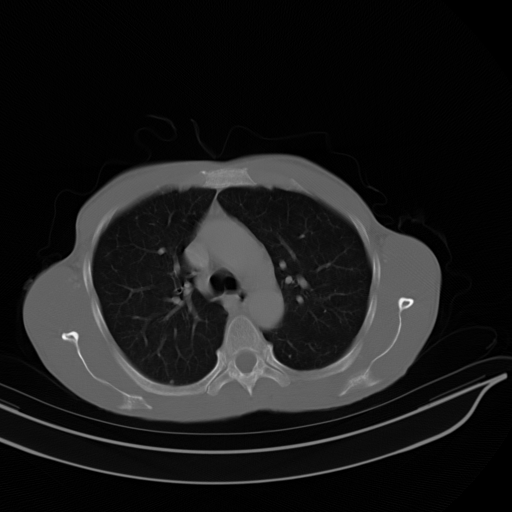
\includegraphics[width=2.9in]{imagens/TCpulmao.png}}
  \subfigure[Depois do threshold adaptativo]{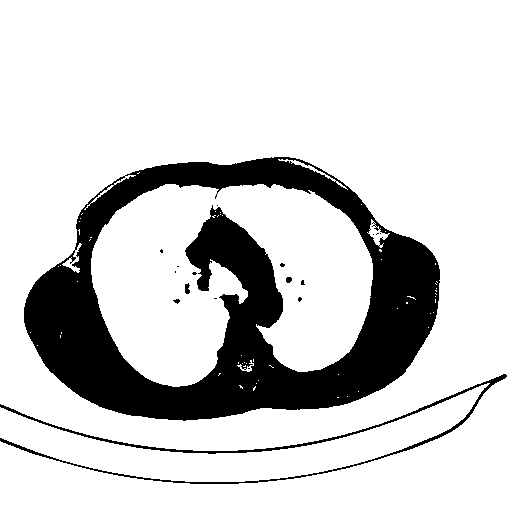
\includegraphics[width=2.9in]{imagens/TCpulmaoTHRESHOLDED.png}}
 \end{center}
 \caption{Imagem de TC original e após a aplicação de threshold adaptativo.}
 \label{fig:threshold}
\end{figure}

\section{Morfologia Matemática}

Morfologia é o estudo da forma. Em processamento de imagens, morfologia matemática é o nome que se dá a um conjunto de métodos, inicialmente desenvolvidos por Georges Matheron e Jean Serra  em 1964, que têm em comum o objetivo de estudar a estrutura geométrica de uma imagem.

A linguagem utilizada na morfologia matemática é a teoria dos conjuntos. Conjuntos na morfologia matemática representam objetos numa imagem. Por exemplo, o conjunto de todos os pixels pretos numa imagem binária é uma descrição morfologica completa da image. Em imagens binárias, os conjuntos em questão são membros do espaço dos inteiros bidimensional - 2D - $Z^2$, onde cada elemento do conjunto é uma tupla cujas coordenadas são as coordenadas de um pixel preto na image. Imagens em tons de cinza podem ser representadas como conjuntos cujos componentes estão em $Z^3$. Neste caso, dois componentes de cada elemento do conjunto se referem as coordenadas do pixel, e o terceiro corresponde ao valor do seu nível de cinza. Conjuntos em espaços dimensionais ainda mais elevados podem conter outros atributos da imagem, como cor ou componentes que variam com o tempo \cite{gonzalez}.

Então temos a morfologia binária que se aplica sobre imagens binárias e a morfologia cinza que se aplica a imagens em níveis de cinza. Uma operação morfológica binária é completamente determinada a partir da vizinhaça examinada ao redor do ponto central e do algoritmo utilizado, Já na morfologia cinza, na vizinhança de cada pixel, ou numa parte da vizinhança, é necessário conhecer o valor do pixel mais escuro, e o valor do mais claro. O valor do pixel resultando corresponde a uma combinação particular desses dois. Portanto o tamanho e a forma da vizinhança, as regiões de pesquisa dos valores máximo e minímo e o algoritmo utilizado, determinam uma operação de morfologia cinza \cite{facon}.

As operações fundamentais da morfologia matemática são a erosão e a dilatação. Essas operações necessitam do que chamamos de elementos estruturantes. Estes elementos, determinam quais pixels da imagem são retirados (no caso de uma erosão) ou quais são adicionados (no caso de uma dilatação) aos objetos. Elementos estruturantes são simplesmente imagens binárias em que um dos pontos é definido como centro. Como exemplos largamente utilizados podemos citar: um quadrado de 3x3 pixels (figura \ref{fig:ee_quadrado}), uma cruz definida pelo pontos {(-1,0),(0,-1),(0,0),(0,1),(1,0)} (figura \ref{fig:ee_cruz}) e um círculo de raio qualquer (figura \ref{fig:ee_circulo}).

\begin{figure}[ht]
 \begin{center}
  \subfigure[Quadrado (3x3))]{
\includegraphics[width=1in]{imagens/ee_quadrado.png}\label{fig:ee_quadrado}}
  \hspace{1.5cm}
  \subfigure[Cruz (3x3)]{
\includegraphics[width=1in]{imagens/ee_cruz.png}\label{fig:ee_cruz}}
  \hspace{1.5cm}
  \subfigure[Círculo de raio 2 (5x5)]{
\includegraphics[width=1in]{imagens/ee_circulo.png}\label{fig:ee_circulo}}
 \end{center}
 \caption{Exemplos de elementos estruturantes.}
 \label{fig:elemento_estruturante}
\end{figure}

\subsection{Erosão e Dilatação}

Na erosão, o elemento estruturante é sobreposto à imagem em todas as posições possíveis. O pixel que fica na posição da origem do elemento estruturante é modificado da seguinte forma: se o elemento estiver em parte sobre o objeto e em parte sobre o fundo, o pixel que está na posição da origem passa a ser fundo. Ou seja, um pixel só pode permanecer no objeto se, quando a origem do elemento estruturante estiver sobre ele, todo o elemento estiver sobre o objeto, como podemos ver na \ref{fig:erosao}.

Efeitos da erosão:

\begin{itemize}
 \item Diminui as partículas;
 \item Elimina grãos de tamanho inferior ao tamanho do elemento estruturante;
 \item Aumenta os buracos;
 \item Separa grãos próximos.
\end{itemize}


Na dilatação o que muda é que quando o elemento está em parte sobre o fundo e em parte sobre o objeto, o seu centro passa a ser objeto, como vemos na \ref{fig:dilatacao}. Isto aumenta o tamanho do objeto, como o nome dilatação sugere.

Efeitos da dilatação:

\begin{itemize}
 \item Aumenta as partículas;
 \item Preenche pequenos buracos;
 \item Conecta grãos próximos.
\end{itemize}

\begin{figure}[ht]
 \begin{center}
  \subfigure[Imagem Original]{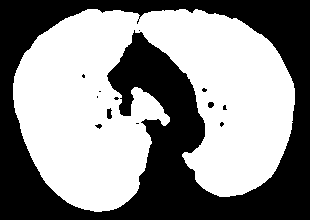
\includegraphics[width=2.9in]{imagens/afterHoleFilling.png}}
  \\
  \subfigure[Dilatação]{
\includegraphics[width=2.9in]{imagens/dilatacao.png}\label{fig:dilatacao}}
  \subfigure[Erosão]{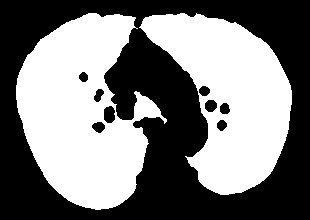
\includegraphics[width=2.9in]{imagens/erosao.png}\label{fig:erosao}}
 \end{center}
 \caption{Imagem de TC após passar por threshold adaptativo e limpeza, submetida a dilatação e erosão utilizando como elemento estruturante um círculo de raio 3 pixels.}
 \label{fig:erosao_dilatacao}
\end{figure}

\subsection{Abertura e Fechamento}

Erosão e dilatação podem corrigir defeitos numa imagem com furos, conexões. Porém, o objeto alterado por essas operações não mantém o mesmo tamanho. A erosão reduz e a dilatação aumenta. Com a abertura e o fechamento binários, podemos manter aproximadamente as características de forma e tamanho do objeto.

A abertura é obtida através da erosão, seguida de uma dilatação da imagem resultante com o mesmo elemento estruturante. Esta operação é capaz de eliminar pequenas partículas inferiores em tamanho ao elemento estruturante quase sem modificar o tamanho das outras entidades, além de nivelar os contornos pelo interior, como podemos ver na \ref{fig:abertura}.

Já o fechamento é o inverso; dilatação, seguida de erosão. Ele conecta partículas próximas, suaviza as bordas pelo exterior e preenche os buracos inferiores em tamanho em relação ao elemento estruturante que estejam no interior das partículas, visto na \ref{fig:fechamento}.

\begin{figure}[ht]
 \begin{center}
  \subfigure[Imagem Original]{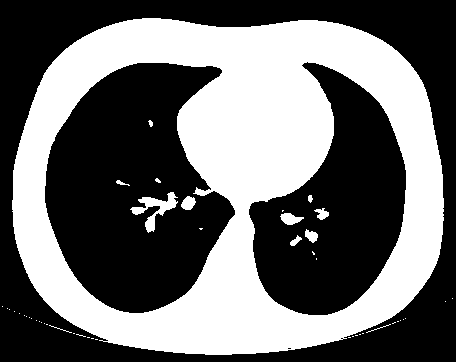
\includegraphics[width=2.9in]{imagens/afterThreshold.png}}
  \\
  \subfigure[Abertura]{
\includegraphics[width=2.9in]{imagens/abertura.png}\label{fig:abertura}}
  \subfigure[Fechamento]{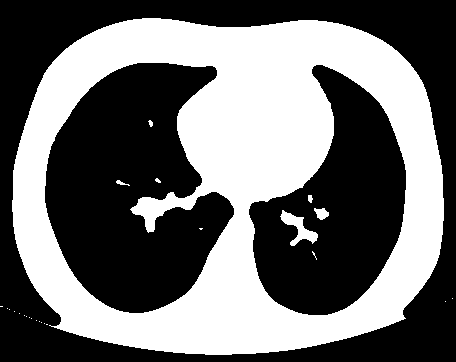
\includegraphics[width=2.9in]{imagens/fechamento.png}\label{fig:fechamento}}
 \end{center}
 \caption{Imagem de TC após passar por threshold adaptativo, submetida a abertura e fechamento utilizando como elemento estruturante um círculo de raio 6 pixels.}
 \label{fig:abertura_fechamento}
\end{figure}

\section{Extração de características de texturas}

O sistema de visão humano percebe uma cena como sendo variações de intensidade e cor, a imagem toda ou as partes dela que formam certos padrões repetitivos, são chamadas de textura. Numa imagem de textura, um conjunto estatístico ou de atributos, varia lentamente ou se mantém quase periódico. Estes atributos, os quais são repetitivos ou quase, dominam as texturas de uma cena.

Uma textura é uma junção de subpadrões que se repetem, que seguem um conjunto de regras de posicionamento bem definido. Estes subpadrões são feitos de unidades mais básicas, chamadas de primitivas. Esta caracterização de texturas é principalmente aplicável a texturas determinísticas, como por exemplo, linhas, tabuleiro de dama, etc. Existem imagens, como imagens de satélite da superfície terreste, que aparentemente não possuem esses padrões básicos que são repetidos ao longo do padrão mais abrangente \cite{acharya}.

Uma imagem que seja uma textura, pode então ser toda reduzida num conjunto de características, também chamado de vetor de características. Essa transformação se chama extração de características. Se as características extraídas forem cuidadosamente escolhidas é esperado que o conjunto de características represente toda a informação relevante da textura.

Uma primitiva é um conjunto conectado de pixels, caracterizado por um conjunto de atributos. A primitiva mais simples é um único pixel com seu atributo de nível de cinza. Um conjunto de pixels conectado que possui o mesmo nível de cinza ou que possui a mesma direção de borda forma uma primitiva. Outros atributos locais podem ser considerados para se definir uma primitiva. Outros atributos incluem a medida de regiões conectadas e a homogeneidade da sua propriedade local. Primitivas podem ser geradas a partir de imagens por vários filtros de vizinhança \cite{acharya}.

\subsection{Matriz de co-ocorrência}

Matriz de co-ocorrência é um dos métodos de processamento de imagens utilizado para caracterizar texturas. Ele descreve uma imagem, ou uma região de interesse na imagem, em termos da relação entre os valores dos pixels com os valores dos pixels vizinhos.

Uma matriz de co-ocorrência é definida a partir de uma imagem como sendo a distribuição dos valores co-ocorrentes num dado deslocamento. Matematicamente, a matrix de co-ocorrência $C$ é definida a partir de uma imagem $I$ de $N x M$, parametrizada com um deslocamento de ($\Delta{}x,\Delta{}y$), como \ref{equa:coocur-matriz}.

\begin{equation}
 C(i,j)=\sum_{p=1}^n\sum_{q=1}^m
 \cases{
	1, & $\mbox{se }I(p,q)=i\mbox{ e }I(p+\Delta{}x,q+\Delta{}y)=j$\cr
	0, & $\mbox{senão}$\cr
 }
 \label{equa:coocur-matriz}
\end{equation}

Para poder ser utilizada, a matriz de co-ocorrência precisa ser normalizada, que poder ser obtida dividindo cada elemento da matriz pelo número total de pares de pixel.

Percebemos que o deslocamento ($\Delta{}x,\Delta{}y$) faz com que a matriz de co-ocorrência seja sensível a rotação. Dessa forma, uma rotação da imagem diferente de 180 graus irá resultar numa matriz de co-ocorrência diferente para uma mesma imagem (rotacionada). Isso é raramente desejado nas aplicações em que a matriz de co-ocorrência é usada, portanto a matriz de co-ocorrência é geralmente usada a partir da média em cada valor da matriz para um conjunto de deslocamentos que variam até 180 graus com uma mesma distância entre eles (por exemplo 0, 45, 90 e 135 graus) para não ser influenciada pela rotação.

\subsection{Características de Haralick}

\cite{Haralick} sugeriu um total de 14 características que podem ser computadas diretamente da matriz de co-ocorrência, as quais podem ser usadas para classificar imagens de textura. Abaixo estão descritas algumas delas.

Considere N como sendo o número de níveis de cinza da matriz de co-ocorrência e.

A Energia, também conhecida como segundo momento angular, avalia a uniformidade textural em uma imagem. A fórmula que descreve a energia pode ser vista em \ref{equa:hara-energia}.

\begin{equation}
 \sum_{i=0}^{N-1}\sum_{j=0}^{N-1} C(i,j)^2
 \label{equa:hara-energia}
\end{equation}

A Entropia mede a desordem em uma imagem, ou seja, o grau de dispersão de níveis de cinza. Ela é calculada como em \ref{equa:hara-entropia}.

\begin{equation}
 -\sum_{i=0}^{N-1}\sum_{j=0}^{N-1} C(i,j) \; log(C(i,j))
 \label{equa:hara-entropia}
\end{equation}

O contraste, mede a presença de transição abrupta de níveis de cinza (bordas) na imagem. Ele é definido como a equação \ref{equa:hara-contraste}

\begin{equation}
 \sum_{x=0}^{N-1} x^2 \left\{\sum_{i=0}^{N-1}\sum_{j=0}^{N-1} C(i,j)\right\},|i - j| = x
 \label{equa:hara-contraste}
\end{equation}

A homogeneidade local, também conhecido como momento diferencial inverso, como o próprio nome sugere, mede a homogeneidade da imagem. Sua fórmula é a equação \ref{equa:hara-homogeneidade}.

\begin{equation}
 \sum_{i=0}^{N-1}\sum_{j=0}^{N-1} \frac{1}{1 + (i - j)^2} \;C(i,j)
 \label{equa:hara-homogeneidade}
\end{equation}

A correlação mede a dependência linear de um nível de cinza em relação aos vizinhos. Ela é calculada como em \ref{equa:hara-correlação}.

\begin{equation}
 \frac{\sum\limits_{i=0}^{N-1}\sum\limits_{j=0}^{N-1} i j\; C(i,j) - \mu_{i}^2}{\sigma_{i}^2}
 \label{equa:hara-correlação}
\end{equation}

Onde $\mu_{i}$ representa a média ponderada, como definido em \ref{equa:hara-media}. Por causa da simetria da matriz de co-ocorrência, não é necessário calcular a média ponderada de $\mu_{j}$. Já $\sigma_{i}$ representa o desvio padrão, como na equação \ref{equa:hara-desvio}, que também se beneficia da simetria.

\begin{equation}
 \sum_{j=0}^{N-1}\sum_{i=0}^{N-1} i \cdot C(i, j)
 \label{equa:hara-media}
\end{equation}

\begin{equation}
 \sum_{j=0}^{N-1}\sum_{i=0}^{N-1} (i - \mu_{i})^2 \cdot C(i, j)
 \label{equa:hara-desvio}
\end{equation}

Além dessas características, também estão definidas em \cite{Haralick}: soma dos quadrados, soma da média, soma da variância, soma da entropia, variância diferencial, entropia diferencial, medida de informação da correlação e coeficiente de correlação máxima.
\chapter{Recuperação de imagens baseada em conteúdo}

Os primeiros trabalhos sobre recuperação de imagens são datados do final da década de 1970. Em 1979, uma conferência sobre \textit{Database Techniques for Pictorial Applications} (numa tradução livre "Técnicas de banco de dados para aplicações com imagens") foi realizada em Florência, Itália. Desde então, o potencial de técnicas de gerenciamento de banco de dados de imagens atraíu a atenção dos pesquisadores.

As primeiras técnicas não foram baseadas em características visuais e sim em anotações textuais das imagens. Em outras palavras, as imagens eram primeiro descritas textualmente, para então serem recuperadas usando busca baseada em texto dos sistemas de gerenciamente de banco de dados tradicionais. Através das descrições textuais, as imagens podem ser organizadas por tópicos ou classes hierárquicas para facilitar a busca através de requisições usando expressões lógicas. Entretanto, como a geração automática de descrições para imagens diversas é uma tarefa quase impossível, a maioria dos sistemas de recuperação baseados em imagem requer que as descrições sejam feitas manualmente. Obviamente, fazer anotações manualmente sobre uma imagem é uma tarefa difícil e onerosa para grandes bancos de dados de imagens, além de ser geralmente subjetiva, sensível ao contexto e incompleta \cite{feng-chapter}.

O objetivo dos sistemas de recuperação de imagens baseada em conteúdo - CBIR (content based image retrieval) - é buscar em um banco de imagens as imagens mais relevantes relativas a uma requisição visual. Dessa forma eliminando a necessidade de descrições textuais manuais e tornando a busca mais eficiente e menos subjetiva.

Num sistema CBIR típico, o conteúdo visual relevante das imagens no banco de imagens é extraído e armazenado como um vetor de características. Para realizar a recuperação das imagens mais relevantes, o usuário fornece ao sistema uma imagem exemplo ou um esboço do que ele busca. O sistema então realiza a extração das características. A similaridade entre o vetor de característica da imagem exemplo ou esboço e cada uma das imagens do banco de dados é então calculada e a recuperação realizada com a ajuda de um esquema de indexação. Sistemas de CBIR recentes levam em conta a resposta do usuário, sobre quais imagens são relevantes, para modificar o processo de recuperação, de forma a gerar resultados mais relevantes.
% TODO: diagrama CBIR típico

\section{Similaridade}

No dia-a-dia precisamos categorizar diversas coisas no mundo real e da informação para que pela comparação com conceitos e situações já existentes, possamos aprender outros. Portanto a capacidade de analisar a similaridade das coisas é importantíssima. Para sistema de CBIR, é necessário que a medida de similaridade chegue o mais perto possível da percepção do usuário, pois ela irá afetar a eficiência das buscas significativamente.

Várias medidas de similaridade foram desenvolvidas para recuperação de imagens nos últimos anos, a maioria baseada em estimativas empíricas da distribuição de características \cite{feng-chapter}. Entretanto essas medidas são estáticas, após escolhidas durante o desenvolvimento do sistema, não são mais alteradas. Dessa forma a utilidade desses sistemas é limitada devido a falta de capacidade de se representar conceitos de alto nível nas imagens utilizando características de baixo nível.

Para contornar esse problema, pesquisadores \cite{mammography} \cite{cbir-nn-general} tem usado para a avaliação de similaridade redes neurais artificiais - RNAs, as quais são capazes de aprender através da interação do usuário.

\section{Redes neurais artificiais}



\section{Relevance Feedback}

\section{Eficiência de um sistema de CBIR}


\chapter{Ferramenta desenvolvida}

Neste trabalho foi desenvolvido um protótipo de ferramenta cujo objetivo é auxiliar na interpretação de exames de tomografia computadorizada dos pulmões. O protótipo, através do processamento de imagens digitais e de técnicas de recuperação de imagens baseada em conteúdo, é capaz de oferecer suporte ao médico na realização do diagnóstico do paciente.

Neste capítulo serão demonstrados aspectos da implementação e utilização do protótipo desenvolvido.

\section{Ambiente de desenvolvimento}

O desenvolvimento do trabalho foi realizado utilizando-se um notebook equipado com processador Intel\textregistered~Core\texttrademark~2~Duo T5450 (1.66GHz), 3GB de memória RAM DDR2 e placa de vídeo NVIDIA\textregistered~GeForce\texttrademark~8400M~GS com 256MB de memória dedicada.

O sistema operacional de desenvolvimento foi o GNU/Linux da distribuição Debian \textit{testing}, utilizando a IDE NetBeans 6.1 com o auxílio das ferramentas cmake, make e gcc.
% WINDOWS XP?

\section{Imagens utilizadas}

% TODO: quem forneceu

% TODO: como foram obtidas, especificações da máquina

\section{Linguagem de programação}

Para o desenvolvimento da ferramenta foi utilizada a linguagem de programação C++. Esta é uma linguagem de alto nível de abstração, com sistema de tipos estático e que permite a programação em múltiplos paradigmas, incluindo programação procedural, genérica e orientada a objetos \cite{stroustrup2000}. Esta linguagem foi desenvolvida originalmente por Bjarne Stroustrup nos laboratórios Bell como uma melhoria para a linguagem de programação C. Dentre as capacidades do C++, destacam-se a possibilidade de fazer abstração de dados, a sobrecarga de operadores e métodos e tratamento de exceções.

Esta linguagem foi escolhida devido a seu desempenho, suporte a orientação a objetos e velocidade de desenvolvimento, além de ser a linguagem nativa da maioria das bibliotecas utilizadas.

\section{Bibliotecas}

Muitas das funções desempenhadas pela ferramenta desenvolvida incluem o processamento e visualização de imagens e gráficos, e ainda a construção, treinamento e utilização de uma rede neural. O desenvolvimento destas rotinas foi escrito com base em algumas bibliotecas que são referência na área por proverem grande quantidade de algoritmos já codificados, testados e prontos para o uso.

% Da mesma forma, a interface gráfica com o usuário também foi construída utilizando funções providas por uma biblioteca escrita por terceiros. Todas as bibliotecas utilizadas no desenvolvimento da ferramenta são distribuídas livremente, com código-fonte aberto.

\subsection{VTK}

O Visualization Toolkit - VTK (Conjunto de Ferramentas para Visualização) - é uma biblioteca voltada à visualização e processamento de gráficos computacionais 2D ou 3D \cite{vtk}. Seu projeto é baseado em técnicas de orientação a objeto e faz uso de bibliotecas gráficas de mais baixo nível, como OpenGL e Mesa3D. Podemos ver alguns exemplos de renderizações na Figura \ref{fig:vtk-ex}.

\begin{figure}[ht]
% TODO: fonte \cite{vtk-page}
 \begin{center}
  \subfigure[Isosuperfícies a partir de dados médicos.]{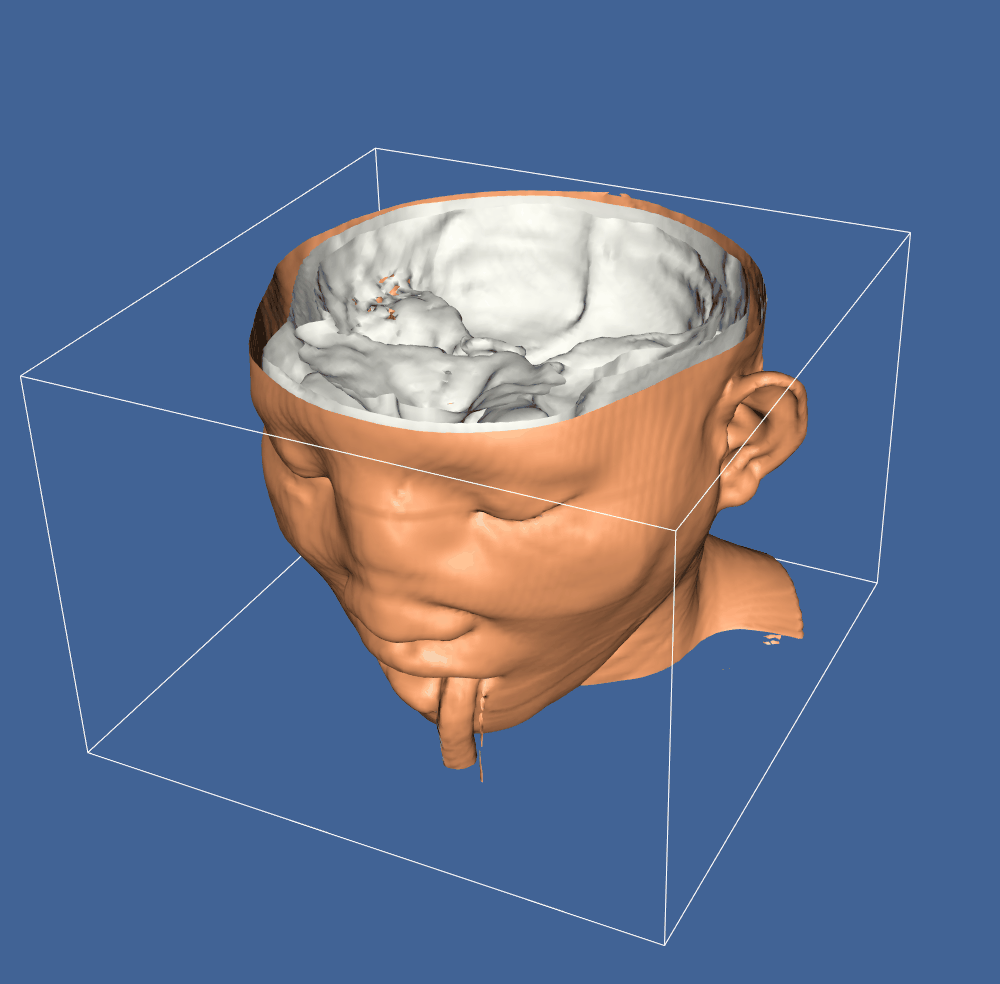
\includegraphics[height=1.9in]{imagens/vtk_ex.png}}
  \subfigure[Visualização de uma função quádrica.]{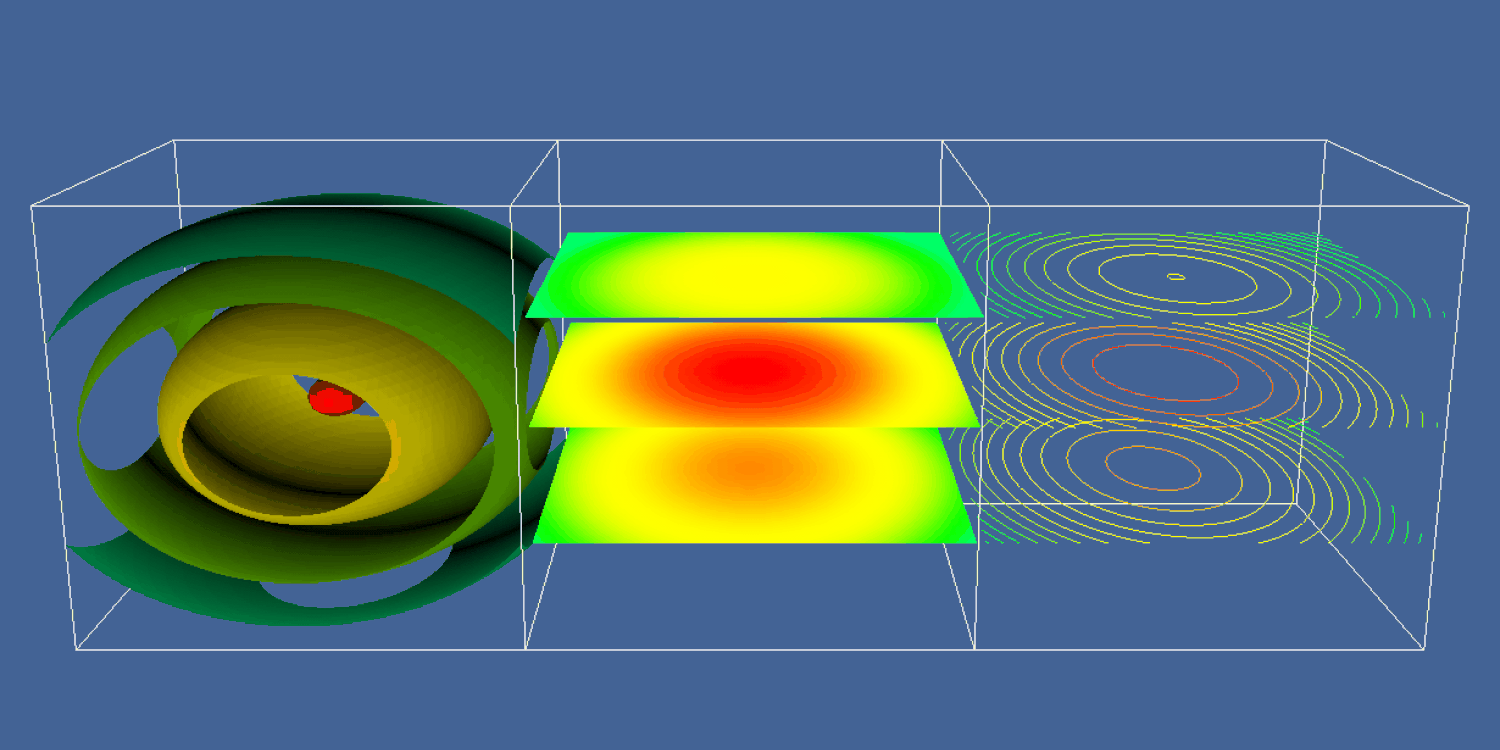
\includegraphics[height=1.9in]{imagens/vtk_ex2.png}}
 \end{center}
 \caption{Exemplos de visualização com o VTK.}
 \label{fig:vtk-ex}
\end{figure}

O VTK é uma biblioteca escrita na linguagem de programação C++, possibilitando a distribuição de classes pré-compiladas, prontas para utilização com esta linguagem. Entretanto, existe um subsistema que consiste de códigos de ligação (wrappers) que permitem a manipulação dessas classes em várias outras linguagens, como Tcl, Java e Python.

Esta biblioteca é independente de plataforma, sendo testada e utilizada em praticamente todos os sistemas UNIX, em Windows 95/98/NT/2000/XP e em Mac OSX Jaguar e versões mais recentes. É utilizado por milhares de pesquisadores, universidades, corporações e institutos de pesquisa ao redor do mundo \cite{vtk-page}.

Por ser um sistema de visualização em um nível de abstração acima de bibliotecas de renderização comuns, permite assim maior facilidade na criação de aplicações gráficas ou de visualização. Esta biblioteca suporta uma enorme variedade de algoritmos de visualização, incluindo os métodos escalar, vetorial e volumétrico. Também inclui técnicas avançadas de modelagem, como redução poligonal, modelagem implícita e triangulação de Delaunay e vários algoritmos para integração de imagens bidimensionais e gráficos tridimensionais.

O processamento dos dados no VTK é feito através de uma arquitetura baseadas em linhas de execução (pipelines). A entrada de dados é conectada sucessivamente em vários filtros e transformações de modo a alterar os dados da maneira desejada e, por fim, ligado a uma classe para visualização.

O VTK é distribuído livremente, com código-fonte aberto e uma licença que impõe pouquíssimas restrições. Entretanto, existe suporte comercial provido pela Kitware Inc., empresa mantenedora da biblioteca.

\subsection{ITK}

O ITK é uma biblioteca proposta pela Biblioteca Nacional de Medicina dos Estados Unidos da América, voltada para segmentação e registro de imagens \cite{yoo}.

O ITK é composto por algoritmos e estruturas de representação de dados com duas finalidades principais: a identificação e classificação de elementos encontrados em uma imagem digital (segmentação) e a tarefa de alinhar imagens ou encontrar correspondências entre dados (registro).

No ITK há um foco em aplicações médicas, embora não haja restrições quanto ao processamento de outros tipos de dados. Essa biblioteca não dá enfoque à parte de visualização deixando a cargo de outras ferramentas que possam ser utilizadas conjuntamente, como o VTK.

O ITK é mantido, basicamente, por seis instituições: Kitware, GE Corporate R\&D, Insightful, University Chapel Hill, University of Utah e University of Pennsylvania, sendo as três primeiras comerciais e as demais são instituições acadêmicas. Outros membros do projeto são Harvard Brigham \& Women's Hospital, University of Pittsburgh e Columbia University \cite{itk-page}.

Quanto à linguagem, o ITK também é escrito em C++, mas possui interface para utilização a partir de outras linguagens. É um conjunto de ferramentas que provê uma grande quantidade de algoritmos pré-codificados e testados para fazer registro e segmentação de imagens, bem como rotinas para leitura e decodificação de diversos padrões de arquivos.

O ITK é também distribuído livremente, com código-fonte aberto e uma licença bem semelhante à do VTK, impondo poucas restrições ao seu uso, modificação e distribuição.

% \subsection{FLTK}

\subsection{FANN}

A FANN é uma biblioteca de RNAs open source. Ela é simples, bem documentada, versátil, fácil de usar e rápida. A FANN é implementada em C, mas possui versões para C++, Java, Perl, PHP, Python, Ruby, Delphi, Haskel, Mathematica, Matlab, Prolog, Octave, Smalltalk e .NET. Ela foi desenvolvida por Steffen Nissen do departamento de Ciência da Computação da Universidade de Copenhagen, que, logo depois, liberou o código sob a licença GPL.

A biblioteca implementa uma RNA de múltiplas camadas totalmente ou esparsamente conectada. Com a FANN, a criação de uma RNA é feita em três níveis. O primeiro é a descrição da rede, o segundo é a criação das conexões da primeira camada, e depois as interconexões das demais camadas. Ela pode trabalhar tanto com números em ponto flutuante quanto números inteiros. Além disso, ela possui um framework para que seja fácil o treinamento a partir de conjuntos da dados.

\section{Algoritmos}

Grande   parte  da   construção    da  ferramenta    foi constituída pelo desenvolvimento de algoritmos que desempenham as funções propostas. A seguir são apresentados, de modo simplificado, cada um dos algoritmos.

\subsection{Segmentação de imagens de tomografia computadorizada dos pulmões}

O objetivo deste algoritmo é gerar a partir de uma fatia da imagem de tomografia computadorizada, duas imagens contendo cada uma apenas um dos pulmões com as partes que não representam ele pretas.

% TODO: normalização da imagem

São 5 as etapas desse algoritmo:
\begin{enumerate}
 \item Realizar um threshold adaptativo, como explicado na subseção \ref{subsec:threshold}.
 \item Subtrair a região que não pertence ao corpo do paciente.
 \item Eliminar pequenas regiões erroneamente marcadas como pulmão pelo threshold.
 \item Eliminar buracos dentro do pulmão e juntar pedaços que possam ter ficado separados.
 \item Identificar cada um dos pulmões e se necessário separa-los.
\end{enumerate}

Para subtrair a região que não pertence ao corpo do paciente, são removidos todos os pixeis que estão conectados e possuem o mesmo nível de cinza dos pixeis da borda da imagem. Como demonstrado na figura \ref{fig:remocao}.

\begin{figure}[ht]
 \begin{center}
  \subfigure[Antes da remoção.]{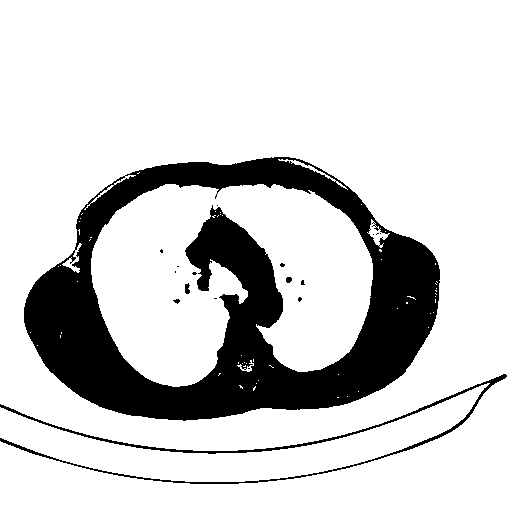
\includegraphics[width=2.9in]{imagens/TCpulmaoTHRESHOLDED.png}}
  \subfigure[Depois da remoção.]{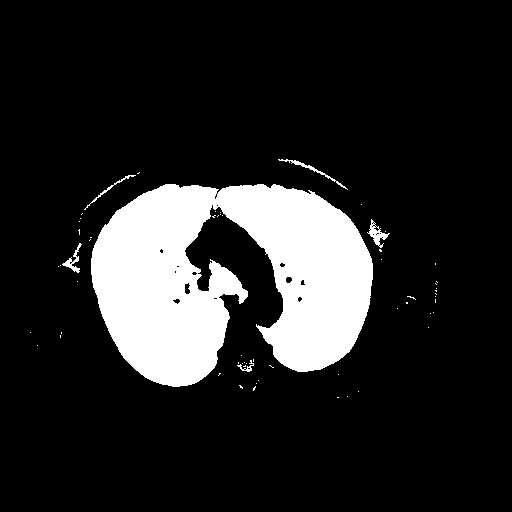
\includegraphics[width=2.9in]{imagens/TCpulmaoWOair.png}}
 \end{center}
 \caption{Imagem de TC antes e depois da remoção das partes que não pertencem ao corpo.}
 \label{fig:remocao}
\end{figure}

A eliminação das regiões que não fazem parte do pulmão é feita analisando-se todos os pixeis que representam o pulmão (brancos) na imagem, de maneira que se a soma dos pixeis vizinhos que representam o fundo (pretos) exceder em 2 ou mais a soma dos pixeis vizinhos que representam o pulmão, então esse pixel se tornará parte do fundo. São considerados pixeis vizinhos aqueles que se encontram no quadrado de 5x5 tendo como centro o pixel analisado.

Esse procedimento é realizado até 40 vezes, ou seja, ele será executado uma vez, se algum pixel for alterado, ele será executado novamente, até que nenhum pixel seja alterado ou que ele já tenha se repetido 40 vezes, podemos ver um exemplo na figura \ref{fig:clean}.

\begin{figure}[ht]
 \begin{center}
  \subfigure[Antes da limpeza.]{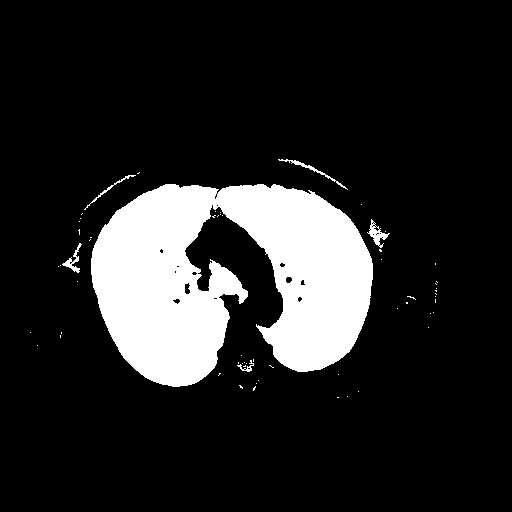
\includegraphics[width=2.9in]{imagens/TCpulmaoWOair.png}}
  \subfigure[Depois da limpeza.]{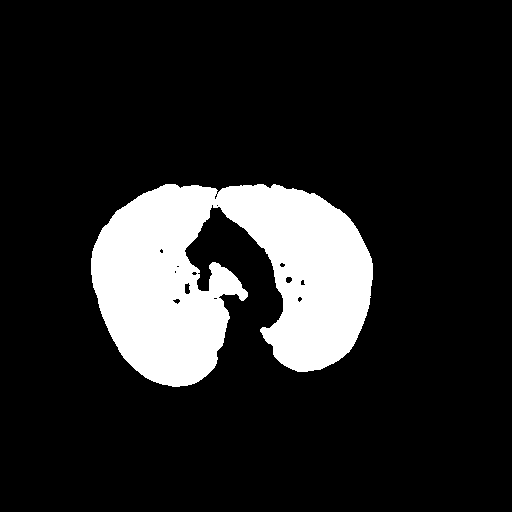
\includegraphics[width=2.9in]{imagens/TCpulmaoCleaning.png}}
 \end{center}
 \caption{Imagem de TC antes e depois da eliminação das regiões que não fazem parte do pulmão.}
 \label{fig:clean}
\end{figure}

Para remover os buracos dentro do pulmão e juntar pedaços separados de um mesmo pulmão, é realizado uma operação morfológica de fechamento utilizando como elemento estruturante um círculo de raio 6 pixeis, como podemos ver na figura \ref{fig:fechamentoAplicado}. Essa operação pode causar com que pulmões muito próximos se juntem, tornando a próxima etapa ainda mais importante.

\begin{figure}[ht]
 \begin{center}
  \subfigure[Antes do fechamento.]{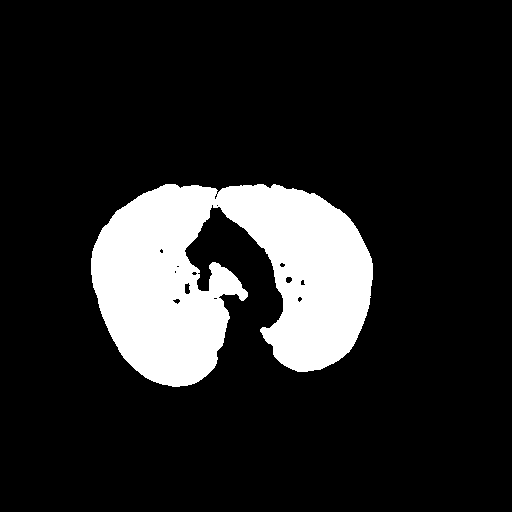
\includegraphics[width=2.9in]{imagens/TCpulmaoCleaning.png}}
  \subfigure[Depois do fechamento.]{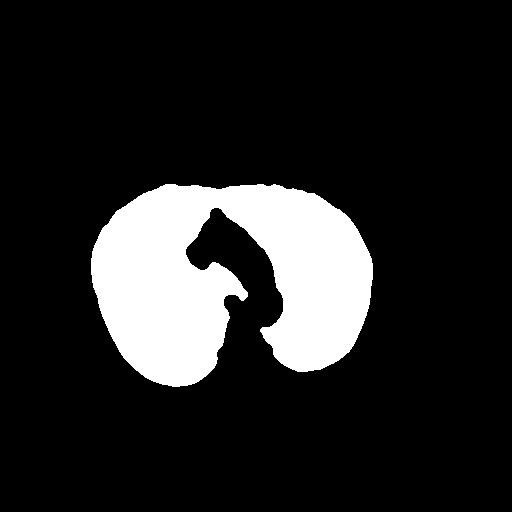
\includegraphics[width=2.9in]{imagens/TCpulmaoBinaryBall.png}}
 \end{center}
 \caption{Imagem de TC antes e depois da operação morfológica de fechamento utilizando um círculo de raio 6 pixeis.}
 \label{fig:fechamentoAplicado}
\end{figure}

% TODO: melhorar
Para identificar os pulmões primeiro verifica-se quantas regiões conectadas existem, se existir apenas uma, realiza-se uma busca a partir do centro da imagem pela coluna que possuir menos pixeis que representam o pulmão, sendo que a busca é parada quando a quantidade desses pixeis aumenta, podemos ver um exemplo dessa etapa na figura \ref{fig:separacao}.

\begin{figure}[ht]
 \begin{center}
  \subfigure[Pulmões juntos.]{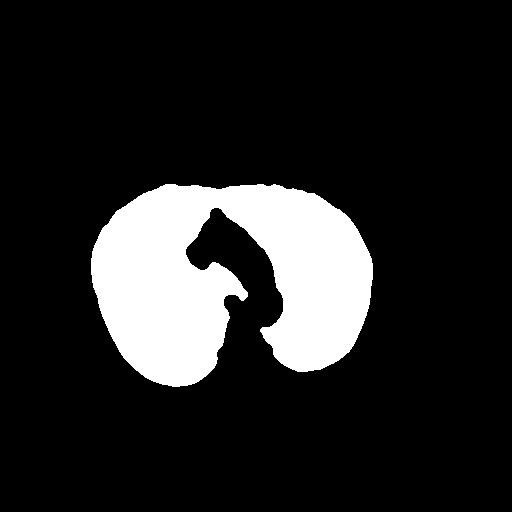
\includegraphics[width=1.9in]{imagens/TCpulmaoBinaryBall.png}\label{fig:separacao:a}}
  \subfigure[Pulmão esquerdo.]{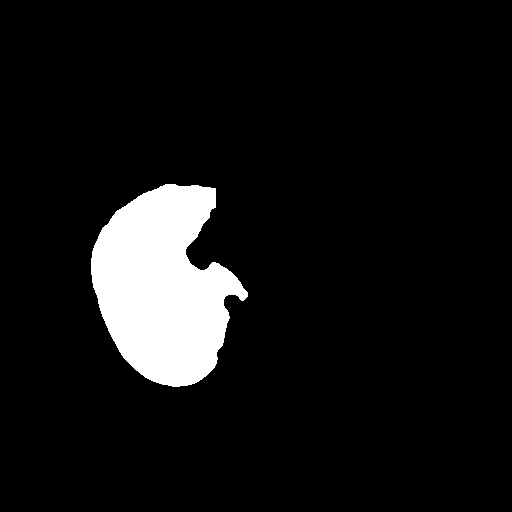
\includegraphics[width=1.9in]{imagens/TCpulmaoEsquerdo.png}\label{fig:separacao:b}}
  \subfigure[Pulmão direito.]{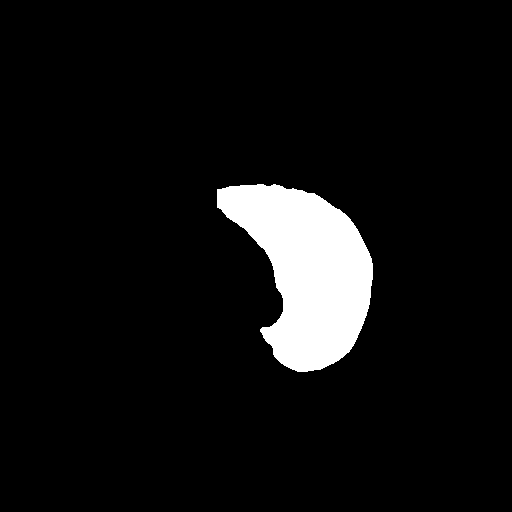
\includegraphics[width=1.9in]{imagens/TCpulmaoDireito.png}\label{fig:separacao:c}}
 \end{center}
 \caption{Pulmões unidos em \ref{fig:separacao:a}, e depois devidamente separados e identificados em \ref{fig:separacao:b} e \ref{fig:separacao:c}.}
 \label{fig:separacao}
\end{figure}

\subsection{Recuperação de imagens baseada em conteúdo}

% TODO: terminar

\chapter{Resultados}

Utilizando imagens de exames cedidas pelo HCFMRP – USP foi possível realizar a segmentação de diversas imagens e realizar o treinamento da RNA através da ferramenta desenvolvida.

\section{Segmentação}

Quanto a segmentação dos pulmões foram observados poucos casos em que o resultado não pode ser usada na etapa seguinte, e geralmente pelas imagens estarem em condições extremas.

Não foi possível avaliar os resultados da segmentação com a opinião de um especialista.

\section{Recuperação das imagens}

Utilizando as imagens disponíveis, a RNA conseguiu identificar as imagens utilizadas no conjunto de treinamento, mas por causa do pequeno conjunto de imagens de cada doença (várias possuiam só uma ocorrência) não foi possível a realização da etapa de teste para medir o erro da RNA. Assim como não foi possível ter acesso a um especialista para que uma avaliação do resultado final fosse feita.
\chapter{Conclusões}

Este trabalho propôs o desenvolvimento de uma ferramenta para auxiliar no diagnóstico de imagens pulmonares de tomografia computadorizada, através da extração de características e recuperação de imagens similares ao exame que está sendo diagnosticado.

Atualmente, está ocorrendo uma expansão na aplicação do processamento de imagens à medicina. Os centros de tratamento médico cada vez mais estão utilizando softwares precisos e confiáveis na análise e diagnóstico de diversas doenças. Como a quantidade de dados coletados por um exame de tomografia geralmente é grande, a utilização de técnicas de processamento de imagens para facilitar a visualização e análise automatizada das informações tem se tornado essencial. É importante ressaltar que este trabalho é o início de um trabalho maior, pois outras características podem ser testadas, além de uma necessidade de aumentar a base de dados, para conseguirmos mais casos de todos os tipos utilizados.

\section{Dificuldades encontradas}

Para a segmentação a falta de documentação e alta complexidade do ITK, associado a quantidade de detalhes do padrão DICOM não implementado por muitas ferramentas, até mesmo no ITK, fizeram com que o tempo de aperfeiçoamento do algoritmo fosse diminuido.

Além disso a dificuldade em encontrar especialistas dispostos a ajudar na avaliação do trabalho não permitiu a validação clínica do mesmo.

\section{Trabalhos Futuros}

Este trabalho pode seguir sendo aperfeiçoado mesmo após sua conclusão. As seguintes metas podem ser destacadas:
\\*
\begin{itemize}
 \item Validar a ferramenta com um profissional a área médica;
 \item Acesso ao laudo das imagens retornadas da busca;
 \item A portabilidade da ferramenta para outros sistemas operacionais;
 \item Utilizar outro conjuntos de características, por exemplo, a técnica de wavelets;
 \item Modularizar a ferramenta de forma a permitir a integração com aplicativos desenvolvidos para segmentação de outros tipos de imagens;
 \item Indicar nas imagens os possíveis locais de patologias;
 \item Utilizar outras topologias de RNA.
\end{itemize}



% TODO: arrumar referencias
\bibliographystyle{abnt-alf}
\bibliography{referencias}

\end{document}
